\section{Overview of neutron \el\ experiments}
\subsection{Neutron detection}
Neutron detection: fast plastic, liquid scintillators, He3 counter, CLYC array, poly
terphenyl. N-gamma discrimination by pulse shape discrimination. TOF techniques
for energy determination. Charged particle rejection. MoNA, neutron wall at
FRIB, VANDAL. Use of machine learning to distinguish gammas from neutrons.

\section{Sample Preparation}
The same \snTwelveNatFour samples used in the neutron \tot\ experiment (see Chapter
\ref{TCSExperiment}) were used for our neutron
\el\ measurements without modification. Two additional samples, one of graphite and one
polyethylene, were provided by the TUNL facility so that our measurements could be benchmarked
against the extremely-well-known (n,p) elastic cross section, described in Chapter \ref{ECSAnalysis}.
The physical characteristics of all the samples are given in \ref{ECSSampleTable}.

\begin{table}[ht]
    \caption[Physical characteristics of samples used for neutron \el\
    measurements]
    {
        For isotopically-enriched samples, the natural abundance
        of the enriched isotope and the isotopic fraction of the sample are
        given.
    }
    \label{SampleCharacteristics}
    \begin{center}
        \begin{tabular}{ c c c c c c c }
            \hline
            Isotope & Length & Diameter
            & Mass & Nat. Abund. & Sample Purity\\
                 & [mm] & [mm] & [g] & [\%] & [\%]\\
            \hline

            $^{\text{nat}}$C & graphite length & graphite diameter & graphite mass & - & -\\
            (CH$_{2}$)$_{n}$ & poly length & poly diameter & poly mass & - & -\\


            $^{112}$Sn & 13.65(3) & 8.245(5) &
            4.9720 & 0.97 & 99.9\\
            $^{\text{nat}}$Sn & 13.68(3) & 8.245(5) &
            5.3263 & - & -\\
            $^{124}$Sn & 13.73(3) & 8.245(5) &
            5.5492 & 5.79 & 99.9\\

            \hline
        \end{tabular}
    \end{center}
\end{table*}

\section{Experimental Facility at TUNL}
We conducted our neutron elastic cross section measurements at the neutron TOF
beamline of the Triangle Universities Nuclear Laboratory (TUNL) facility
(diagrammed in Fig. \ref{ExperimentalSetupTUNL}). Incident deuterons, supplied by the
facility's variable-energy tandem Van De Graaf accelerator, impinged on a deuterium
gas cell to produce a forward-focused neutron beam via the d(d,n)$^{3}$He reaction.
Given the beam profile, the neutron energy distribution was calculated as [insert beam energy
distribution] MeV with a FWHM of [insert beam energy distribution FWHM] MeV for the
11 MeV and 17 MeV experiments, respectively. The gas cell was backed with a fresh tantalum
beam stop to prevent unreacted deuterons from reaching the samples. 

The production samples (\snTwelve, \snFour, and a blank) were suspended in a
vertically-aligned wire basket [insert distance] cm
downstream of the gas cell. Between runs, they were rotated into position
with a hand-actuated pulley, with
alignment confirmed by telescopic sight coaxial to the beam.
Neutrons scattering off the samples were recorded by one of the two main time-of-flight
detectors, labeled ``4M" and ``6M", roughly 4 and 6 meters away from the target.
These detectors were mounted on large, movable carriages, or "arms",
that could be rotated to different angles independently so that two angular
measurements could be conducted simultaneously. By recessing them deep within
the arms' heavy shielding, the detectors were only accessible to neutrons
entering the arm at a precise angle.

%The distance of the 4M (6M) angular
%detector from the sample was X (Y) cm, which, for an elastically-scattered
%11 MeV neutron, corresponds to a [insert time] ([insert time]) ns time-of-flight.

To further reduce room background and prevent neutrons from entering the arms directly
from the gas cell, an ensemble of "shadow bars" (wedge-shaped tungsten bricks)
were used to adjust the aperture at the entrance to the arms. After an arm's
angle was changed, the shadow bars were aligned by hand so that the
detector deep within the arm had no line-of-sight to the gas cell or the
shielding of the other arm, but it maintained line-of-sight to the entire sample volume. Any 
configuration in which the arms were in opposition (i.e., the
angle between the arms was 180$\pm$20 degrees) could allow neutrons scattered
from one arm to enter the detector of the other arm, so these
configurations were avoided.

\begin{figure}[h]
    \centering
    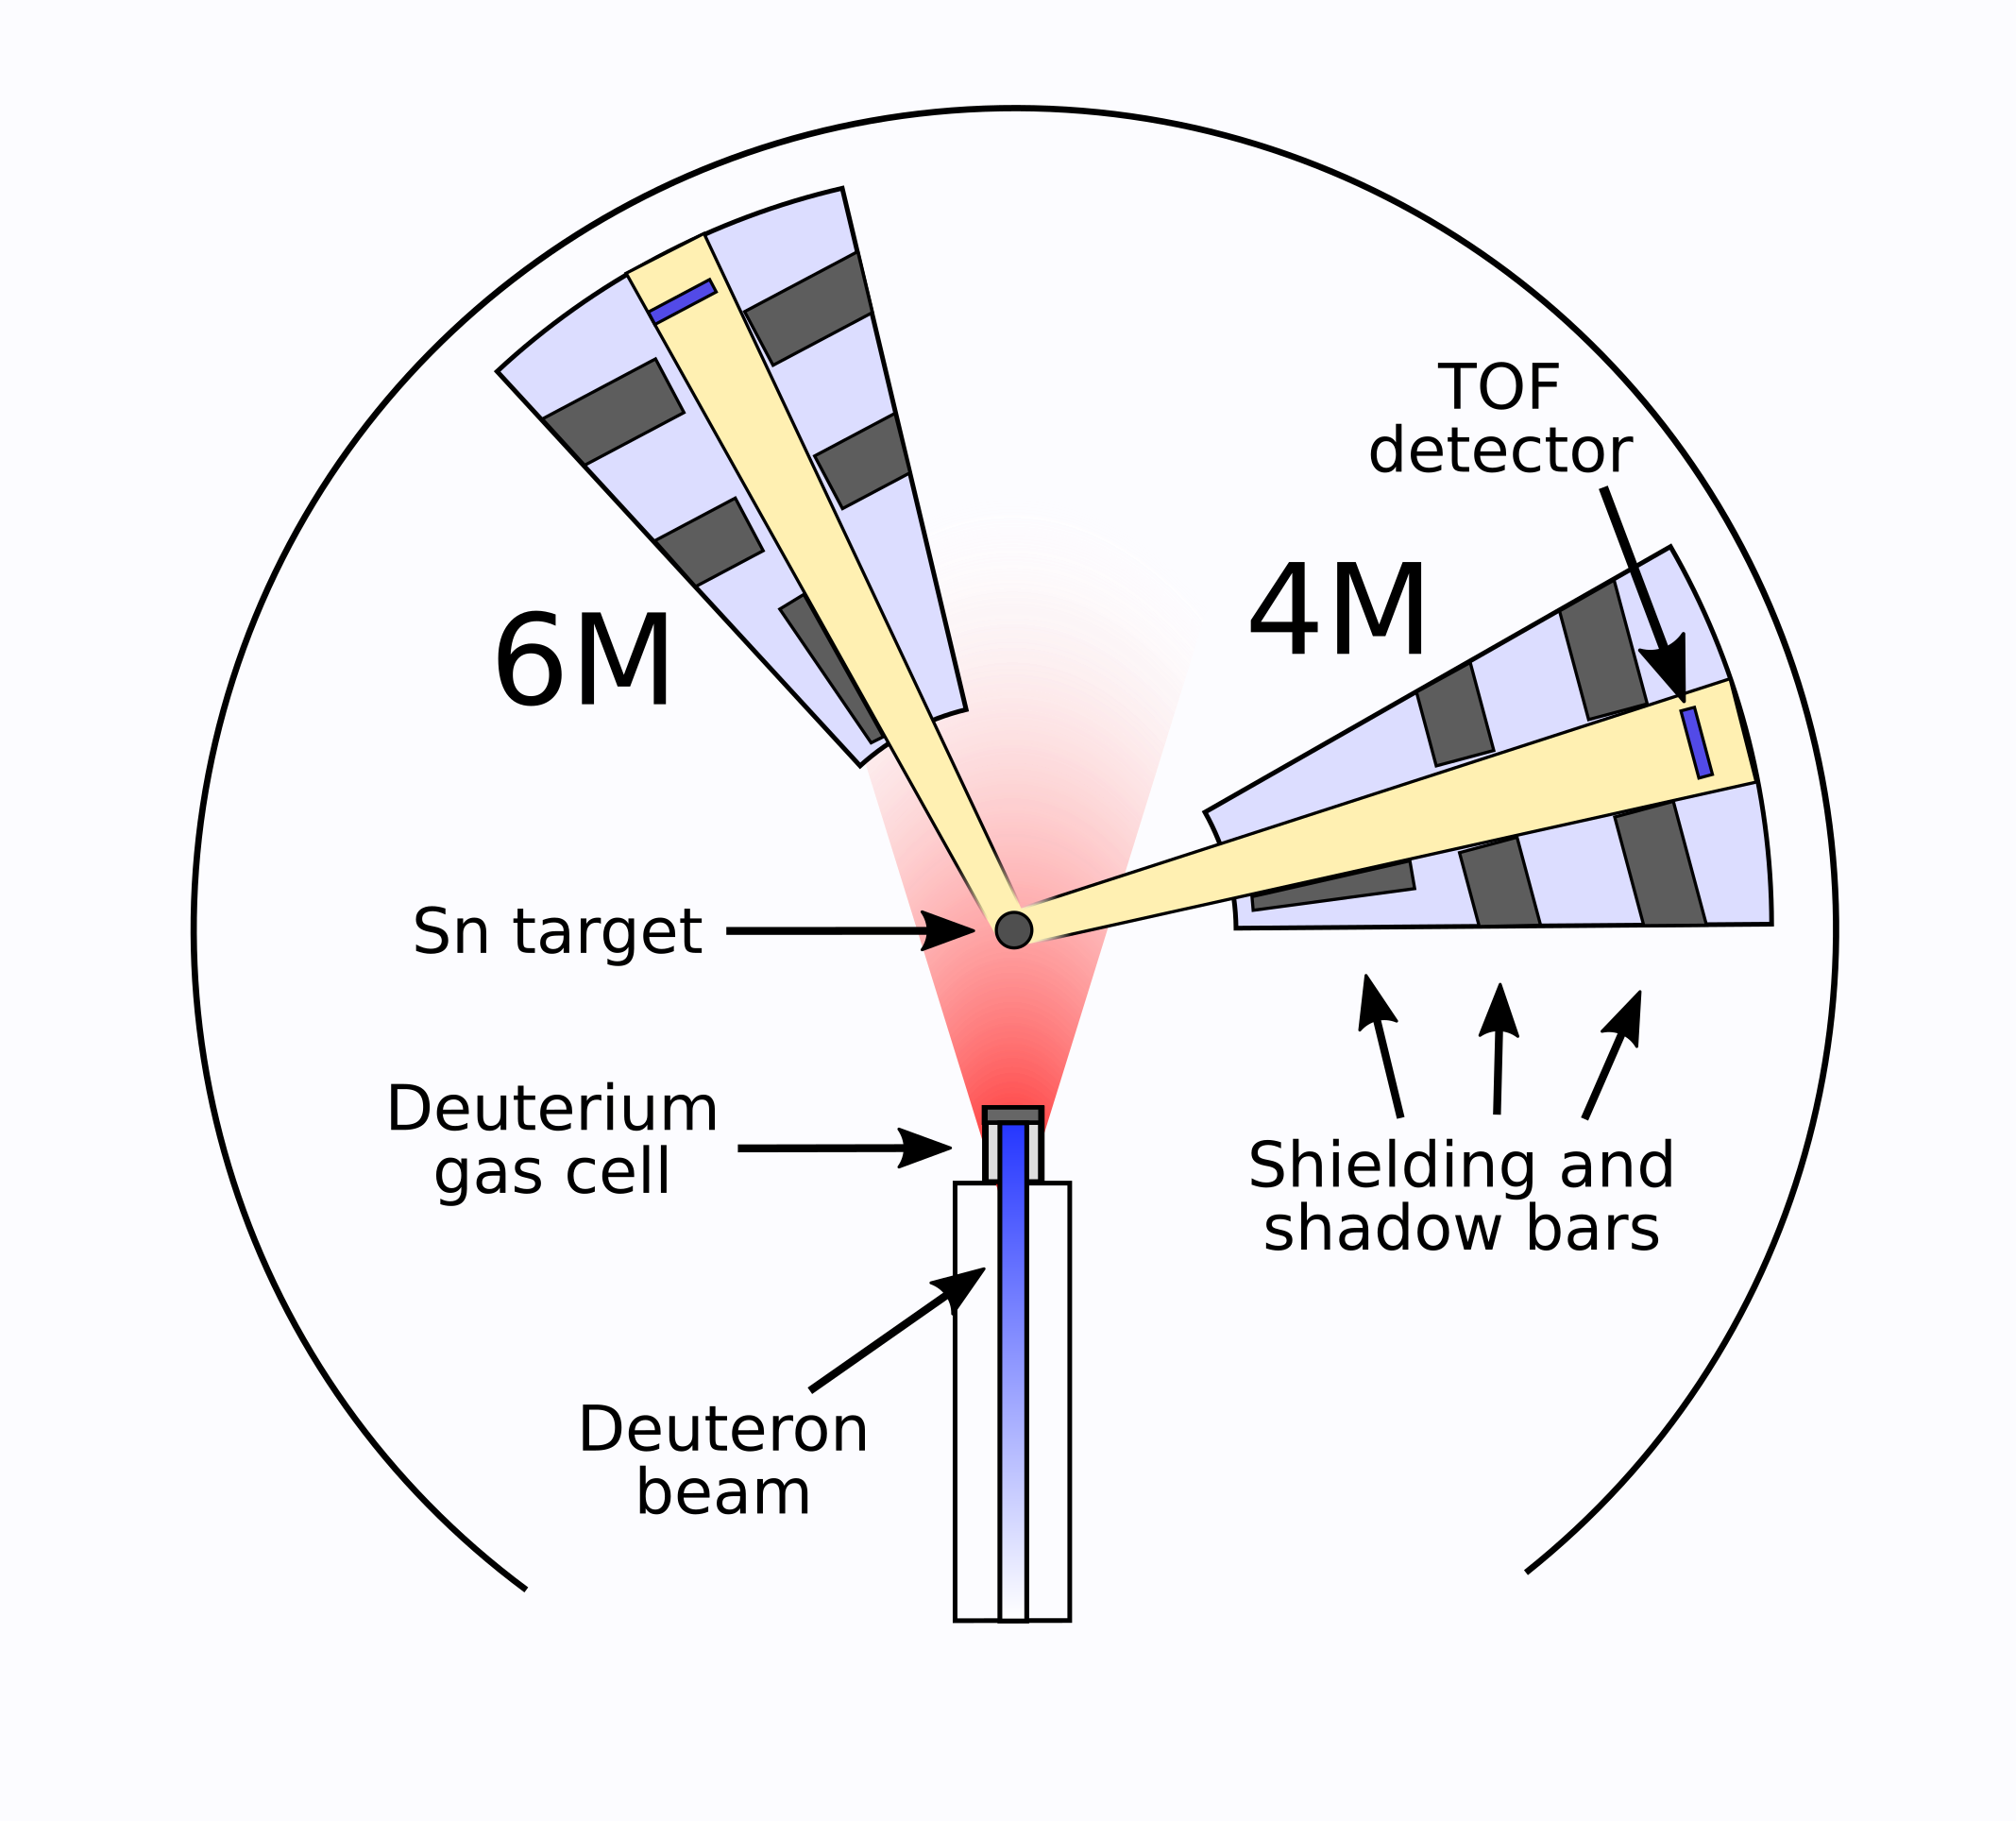
\includegraphics[width = 0.9\textwidth]{figures/ExperimentalSetupTUNL.png}
    \caption[Diagram of the neutron TOF room at TUNL] 
    {
        Diagram of the neutron TOF room at TUNL. Neutrons are produced by d(d,n)$^{3}$He reaction in
        a small gas cell, forming a forward-focused cone (in red). They scatter
        off the sample into one of the detector arms, labeled 4M and 6M, where the neutron
        times-of-flight are recorded. Another shielded detector (not pictured), suspended from the 
        ceiling, serves as a flux monitor so that absolute cross sections can be recovered.
    }
    \label{ExperimentalSetupTUNL}
\end{figure}

\begin{figure}[h]
    \centering
    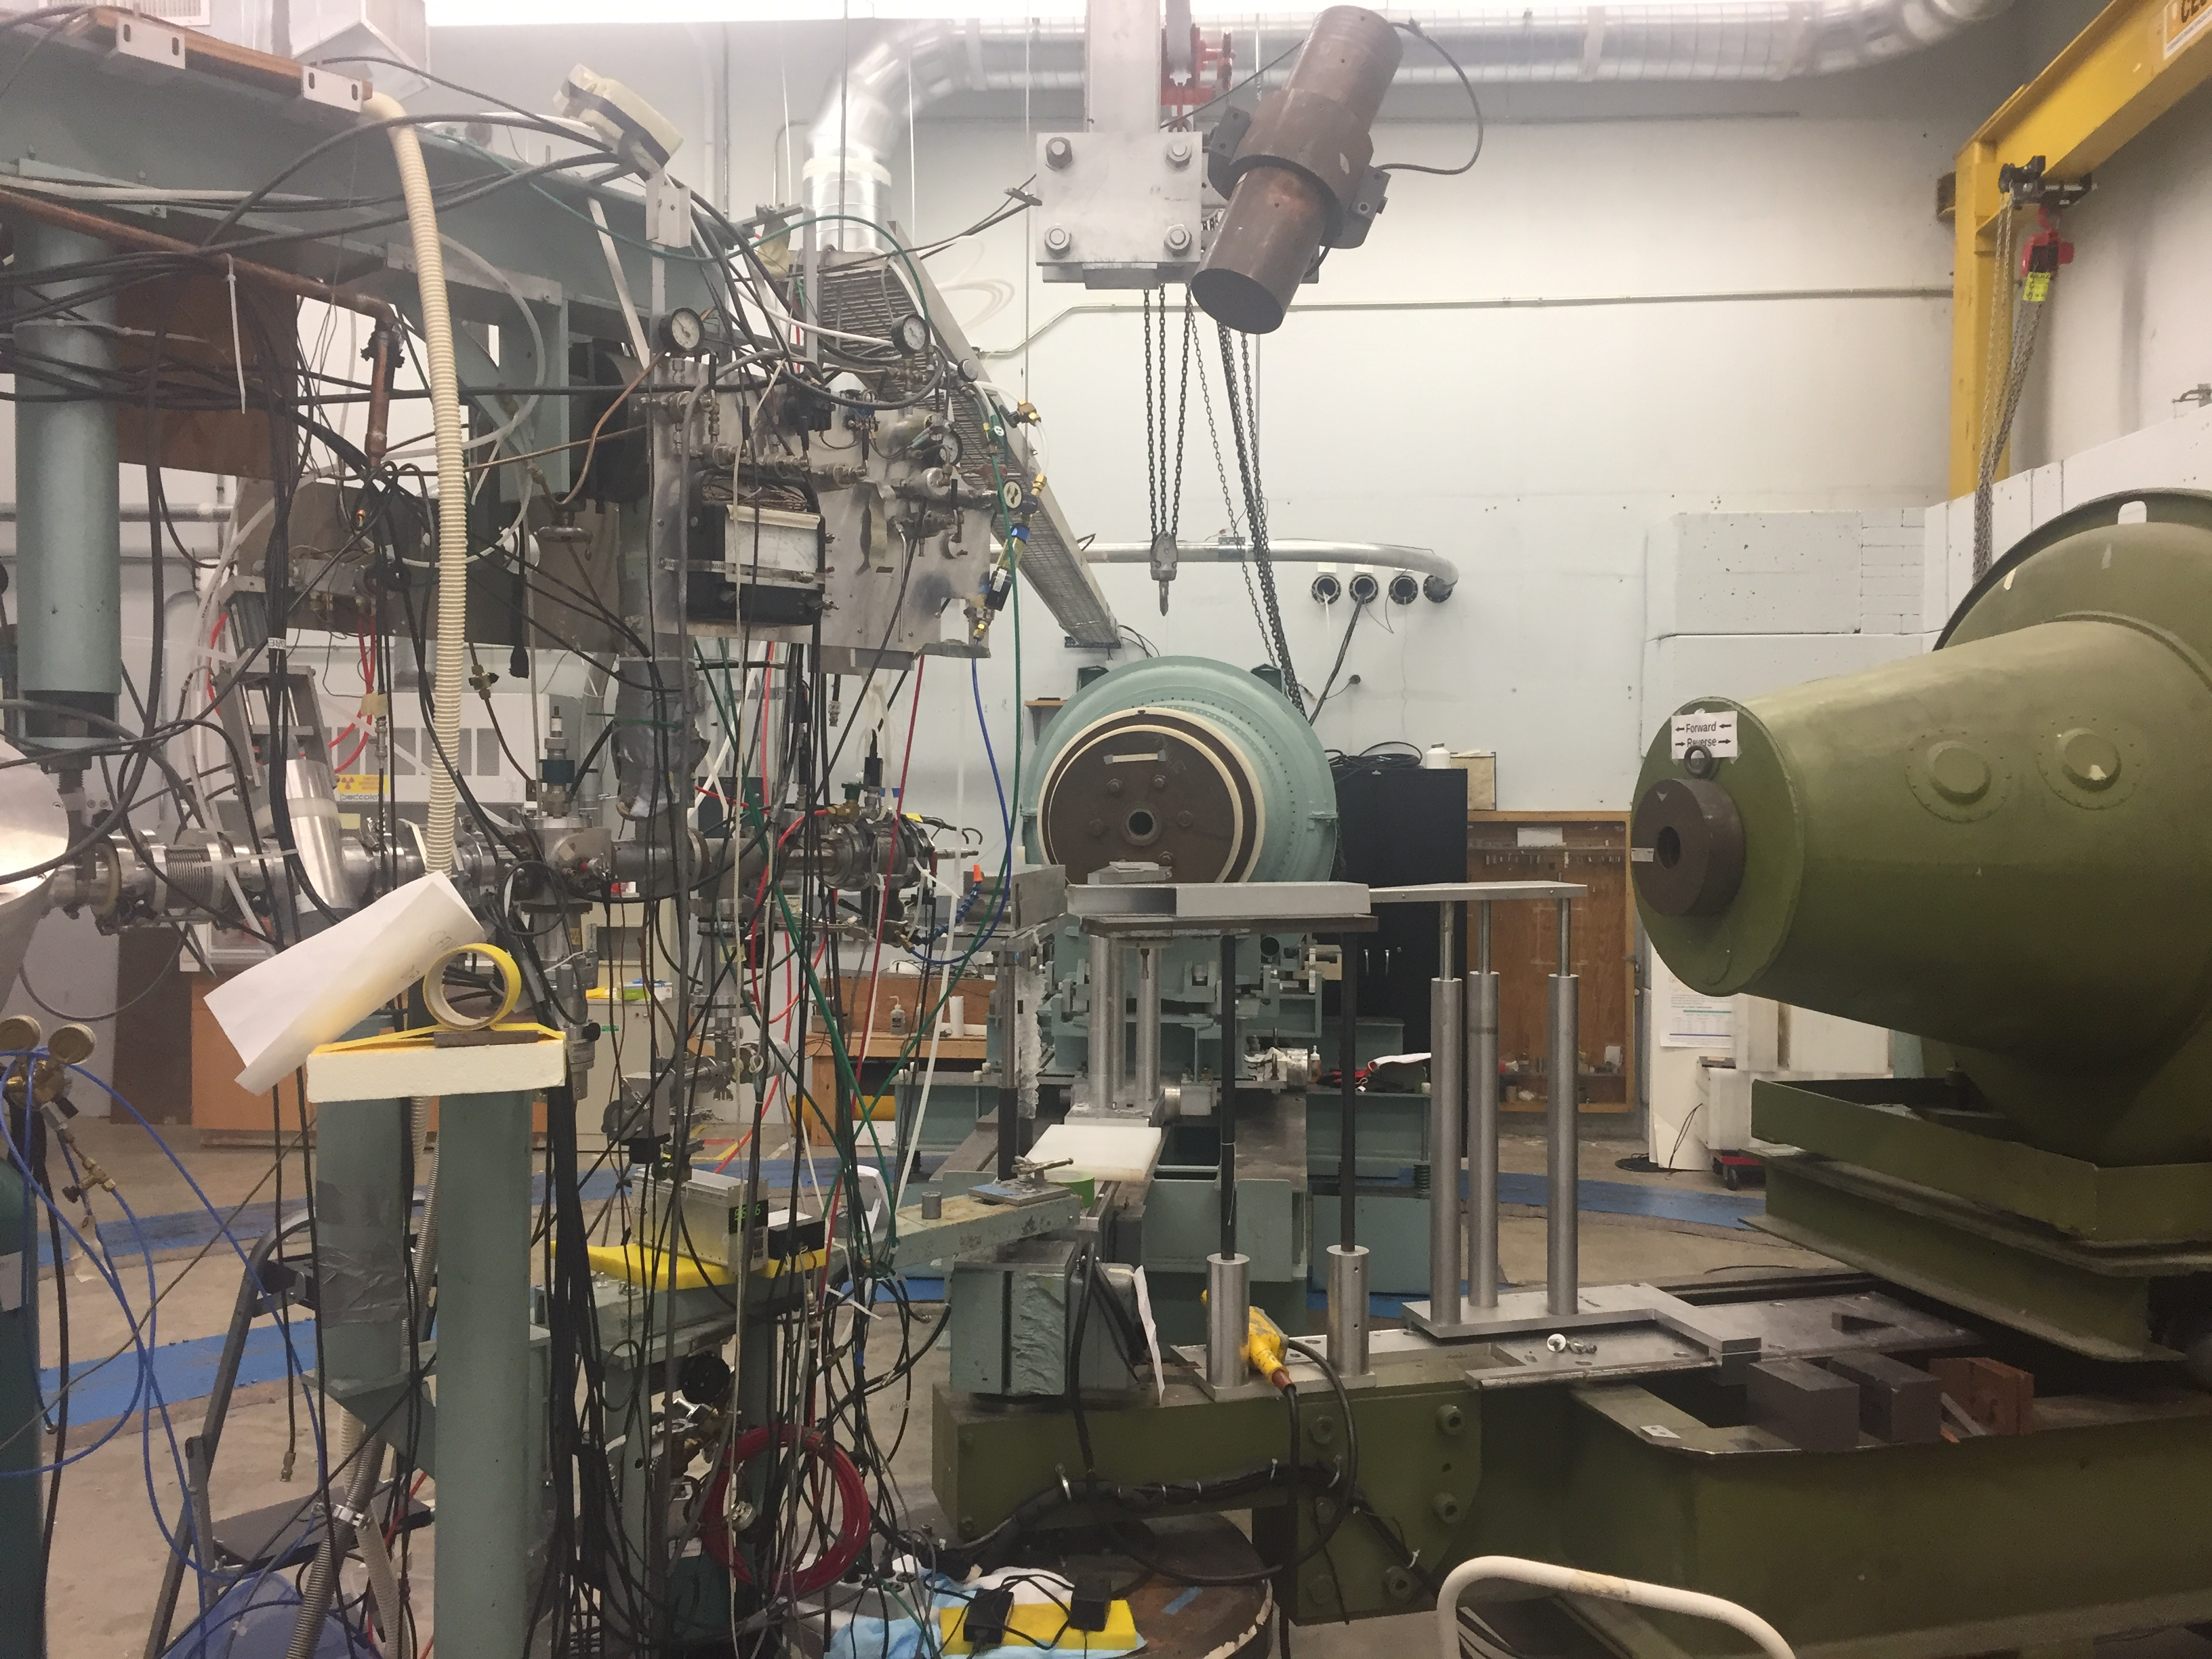
\includegraphics[width = 0.9\textwidth]{figures/TOFRoomPhoto.jpg}
    \caption[Image of the neutron TOF room at TUNL] 
    {
    Image of the neutron TOF room at TUNL. The deuteron beam pipe is visible on the left and
    terminates in a small deuteron gas target in the middle of the image, where neutrons are
    produced. The two goniometric detector arms are shown at center (6M) and right (4M). The ceiling
    monitor detector (CMON), which records beam flux, is visible at the top of the image.
    }
    \label{TOFRoomPhoto}
\end{figure}

Signal timing and pulse shape data were collected from four [liquid scintillator]
detectors: one in each of the angular arms, one in a ceiling monitor
(CMON), and one at zero degrees with respect to the beam (ZDEG). In addition,
an RF pulse from the accelerator was collected to serve as a time-of-flight
(TOF) stop signal any time an event was recorded on one of the four neutron
detectors. Detector gain was calibrated with $^{137}$Cs and $^{22}$Na sources. For
the 4M (6M) detector, a time resolution of X (Y) ns was established.

\section{Data Acquisition}
Signals from all detectors were fed into [insert logic]

\begin{figure}[h]
    \centering
    \includegraphic[width=0.9\textwidth]{figure/ECSLogic.png}
    \caption[Logic diagram for neutron \tot\ data acquisition]
    {Details on logic diagram}
    \label{ECSLogicDiagram}
\end{figure}

